\documentclass[11pt,twocolumn]{article}
\usepackage{graphicx}

\begin{document}

\title {Why robot programming is hard}
\author {Tessa Lau \\
Willow Garage \\
Menlo Park, CA USA \\
{\tt tlau@willowgarage.com}
}
\maketitle

I never thought I would be a roboticist. In grad school, our robotics team spent months teaching little robot dogs to play soccer and solving other seemingly simple problems. Far better to work in the world of software, I figured, where the systems I built could make a real difference in people's lives. Software could automate repetitive tasks in computer use and free people from mundane work. My chosen field, end user programming, had the potential to enable millions of ordinary computer users to customize and adapt systems to their own needs.

But the world is changing. Computing has moved off the desktop and into the smartphones, smart environments, and the world around us. Innovation is happening in the physical world, using computing to effect material change in our environment. The past decades have seen industrial robots increase manufacturing efficiency on the factory floor. Even more, we are now seeing robots tackle tasks from our daily lives. Robotic vacuum cleaners are changing the way we clean our homes. Robotic lawnmowers keep the yard tidy without having to lift a finger. Nest's robotic thermostat learns your habits and keeps your home at the optimal temperature. Google's driverless car could change the way we commute.

All these innovations have become possible through multiple advances: in sensor technology, which robots use to perceive the world around them; in planning and navigation, which enable robots to move around in the world unaided; in human-safe motion controllers, which let robots move their limbs without endangering the people around them; in the ROS open source robot operating system, which enables roboticists to build on each others' work without starting from scratch; and many more advances in the broader field of robotics.

Yet the holy grail of personal robotics remains elusive. When will we have our own Rosie the Robot to take over housekeeping chores? When will disabled adults have robot helpers to assist them in activities of daily living? All of these advances in robotics still fall short of the goal of creating personal robots that can do whatever we want them to do.

What I have found is that the problem is not that robots {\em cannot} do what we want them to do. The problem is that it is too difficult to {\em tell} robots what we want them to do. Robot control can be roughly categorized into three distinct phases: direct demonstration, tele-operation (or teleop for short), and higher-level programming.

In demonstrational interfaces, a human operator moves a robot through a series of positions to demonstrate the motion it should perform. The robot then continues to perform this motion unattended. This style of programming is common for industrial robots, which can be programmed to move items around on conveyor belts or do precise assembly tasks. Demonstrational interfaces are typically limited to repeating only what was previously demonstrated, in the worst case performing the exact same motion down to the millimeter regardless of whether the part is in the same place as it was last time.

Teleop consists of synchronously controlling a robot using software and hardware interfaces from a computer which may or may not be co-located with the robot. For example, a PS3 joystick controller could be used to drive a robot around a building, and activate certain pre-programmed motions such as turning its head or extending its arms. Remote teleop consists of controlling the robot over a distance, perhaps over the internet, using GUIs that allow the human operator to move various parts of the robot.

Both demonstration and teleop suffer the limitation that a human operator must be immediately in the loop while the robot is operating. To make robots useful in the home, they will need to function {\em autonomously}, which leads to the notion of robot programming: giving high-level directives to robots so that they can function on their own without direct human guidance.  A full programming solution will likely involve a blend of different techniques including demonstration, teleop, and autonomous subroutines. For example, a task of setting the dinner table may include a high-level program of fetching silverware from the kitchen and placing it on the dining table, a demonstration of how to open this particular silverware drawer, and teleoperation when something goes awry (such as the silverware drawer being empty).

For personal robotics to truly succeed, robot programming will need to be simple enough that non-experts can do it.

\section{Case study: Robots for Humanity}

One important use case for personal robotics will be in-home care and assistance for disabled adults. The Robots for Humanity project~\cite{rfh}, a collaboration between Willow Garage and Georgia Tech, aims to develop technology that enables persons with motor impairments to perform personal care tasks that they otherwise might not have been able to perform without assistance, such as picking up a dropped object, fetching a towel, or even scratching an itch. Its first prototypes have enabled Henry Evans, a mute quadriplegic, to act in the world for the first time since a brainstem stroke left him paralyzed. Through physical therapy, Henry has regained the ability to make limited head motions (enough to control a cursor with his gaze) and to click a button with one finger.  Using a teleop interface custom designed for him, Henry has been able to instruct Willow Garage's PR2 robots to open cabinets in his home, fetch food from the refrigerator, and even dole out candy to trick-or-treating kids on his behalf.

% TODO: conflating robot programming with teleop

Yet our experience with Robots for Humanity underscores how difficult it is for ordinary mortals to instruct robots what to do. Even using state-of-the-art robot visualization software developed at Willow Garage, simple teleoperation tasks such as opening a cabinet door could take Henry upwards of 15 minutes to accomplish.  While Henry has only limited interaction capabilities, he is also strongly motivated because he has no alternatives. Able-bodied consumers, on the other hand, would quickly lose patience. If even basic robot control via teleoperation is so time-consuming, what hope do we have that people will ever get around to the general task of robot programming?

Granted, designing teleoperation interfaces for motor-impaired users is deliberately trying to solve the hardest problem first.  Yet while Henry's case highlights the challenges of creating usable assistive robotics interfaces, it also illustrates the enormous benefit to humanity of enabling disabled adults to regain some of their independence.

With this goal in mind, autonomous programmable robots are more than a consumer toy, but a technology that could changes people's lives for the better. Why, then, does robot programming for the masses remain such a difficult challenge? What makes robots so difficult to control?

The explanation begins with a look at the state of the art in robot software today.

% Until users are able to instruct robots quickly and with low effort, personal robotics will be limited to niche markets.  Why is end user robot programming so challenging? Several compounding factors make it more difficult than normal computer use.

\section{The state of the art}

% History of ROS
% Invented by Willow Garage, new operating system for diverse robots
% Current reach
% Running on robots from PR2 to android-powered XXX
% Provides very rich control substrate for programming the behavior of complex robots

The Robot Operating System\cite{ros} is one of the software advances that supports the rapid development of new robotics technology.  First developed in 2007 at the Stanford Artificial Intelligence Laboratory, ROS was maintained by Willow Garage from 2008-2013 and has recently transitioned into the stewardship of the non-profit Open Source Robotics Foundation.

ROS provides a distributed publish/subscribe messaging platform for a collection of {\em nodes} to communicate with each other. Each node encapsulates a small amount of robot functionality, and interfaces with the rest of the ROS ecosystem to make that functionality available through a common interface. For example, ROS nodes exist to stream sensor data from webcams and laser rangefinders, control the motors in robot arms, plan a path from one point to another, and recognize graspable objects in an image.

Before ROS, roboticists had to create the software to control their robots from scratch, each doing the same work to create device drivers and rebuild libraries for their specific robot's hardware.  Now, ROS has been ported to around 100 different models of robots worldwide\footnote{http://www.ros.org/wiki/Robots}, enabling roboticists to quickly bring a new robot model online.

\begin{figure*}[tbh]
\center\scalebox{0.20}{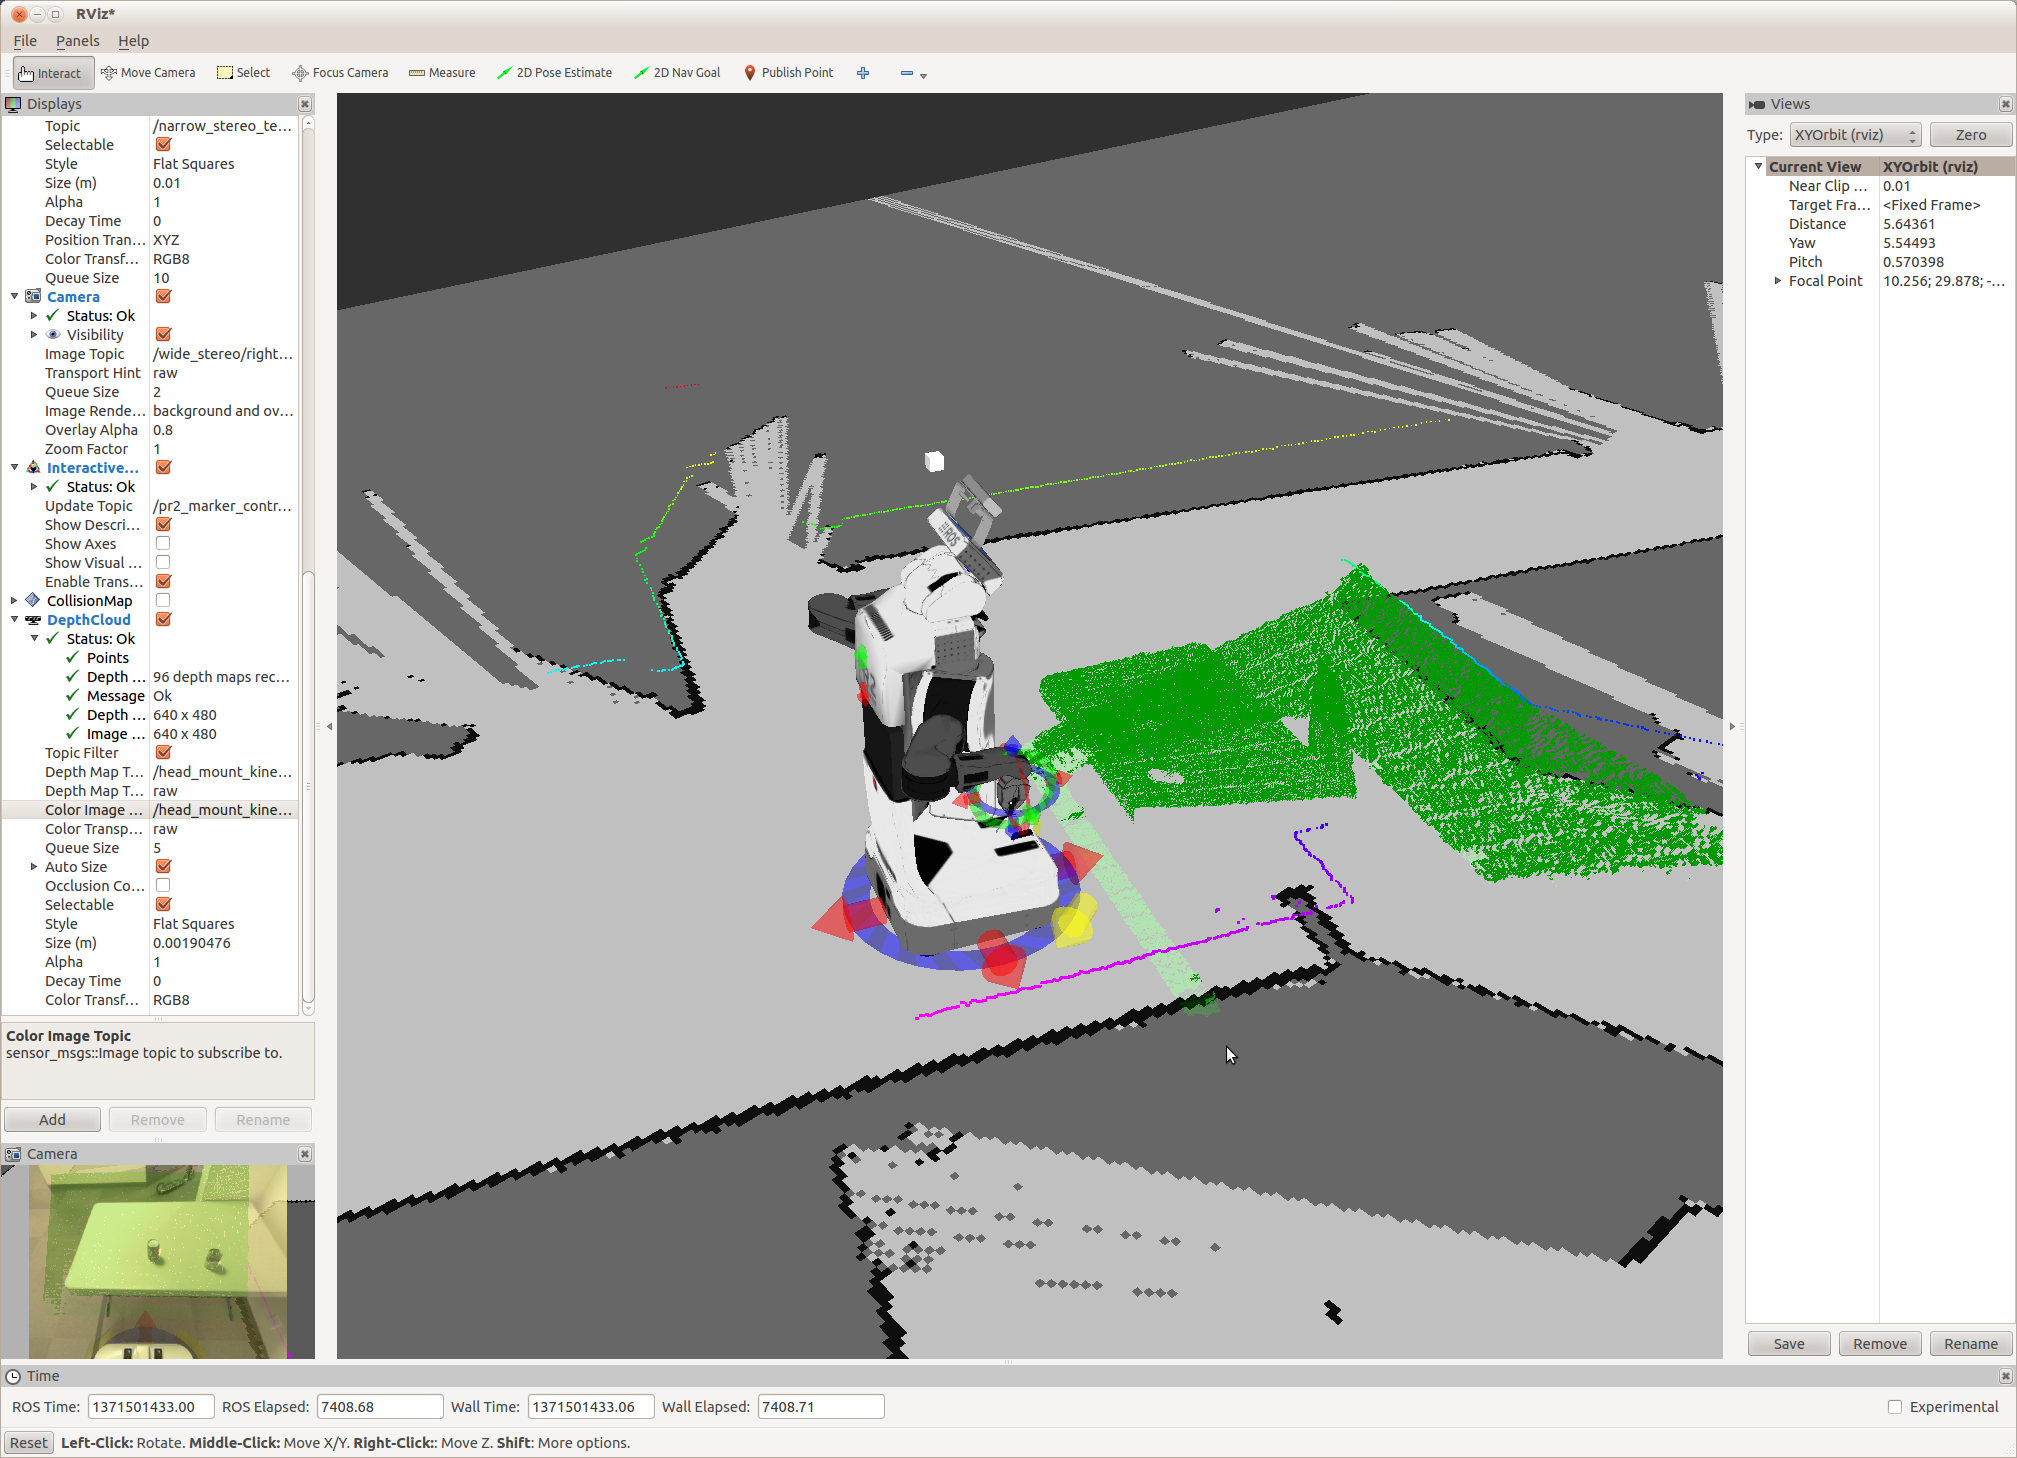
\includegraphics{rviz.png}}
\caption{RViz interface for controlling robots}
\label{rviz}
\end{figure*}

However, ROS provides a fairly low-level interface to robot control. Designed for roboticists, the RViz interface (Figure~\ref{rviz}) displays all the sensor feeds coming from the robot and lets one send low-level motion commands to the robot such as rolling forward or rotating the shoulder joint. In the figure, a robot is shown examining objects on a table in front of it. The green pattern represents the data from a depth sensor mounted on the robot's head, whereas the purple line represents the walls detected by a laser rangefinder mounted on the robot's base. The tricolored axes display the various coordinate frames in use, and the gray floor displays the map the robot uses for navigation. (TODO: display costmaps, TF axes)

This interface, while well suited for roboticists who need to examine the low-level sensor data and messages being processed by the robot, is not very user-friendly. It also illustrates some of the difficulties inherent in robot programming.

\section{A 3D world}

% Robot arms have 7DOF
% grasps require 6D
% world is 3D
% quaternions, matrix manipulation
% specialized I/O devices

Unlike traditional computer interfaces which are limited to two dimensions, robot control requires manipulating objects in a three-dimensional world. Visualizing a 3D world on existing 2D displays requires the extra dimension to be projected down into two dimensions, giving rise to the popular ``first person shooter'' style of interface. These interfaces display the world as perceived from a virtual camera, where objects can be occluded by other objects. Additional camera controls are needed to pan/zoom around the space to overcome occlusion. These controls are often non-intuitive, even to seasoned computer users.

Occlusion presents a challenge because robots must perceive an object in order to manipulate it.  Often times, the robot itself might occlude the object it is trying to manipulate! For example, consider a humanoid robot with head-mounted vision sensors using an arm to pick up an object from the table in front of it. While moving the arm into position to grasp the object, the arm will likely come between the head and the object, obscuring the robot's vision.

One solution has been to mount additional cameras on different parts of the robot, such as on the robot's forearm or wrist, to get a better view on the object being picked up. However, making sense of multiple translated and rotated video streams can be confusing for those of us accustomed to perceiving the world only through head-mounted eye sensors!

Typical input devices such as mice and touchscreens are also only good for interacting in two dimensions. For example, tapping on a point in a camera image does not uniquely identify a point in 3D space, but a line of possible points. When telling a robot to put something down, how can it know which of those points was meant? Current interfaces, such as the RViz display shown in Figure~\ref{rviz}, require complex camera manipulation and precise 3D positioning in order to uniquely specify the desired location.

\section{Arm complexity}

A different aspect of high-dimensionality comes from the design of robot arms. A solid object in 3D space has six degrees of freedom (DOF): three dimensions to specify its position, and three more to specify its rotation. If a robot arm had only 6-DOF and was trying to execute a specific grasp of a particular object, such as picking up soda can from the side, there would be only a single arm configuration that would allow the gripper to pick up the can. In contrast, human arms and advanced robot arms have 7-DOF, which allows them one extra dimension of flexibility in achieving those grasps. To visualize this, imagine grasping a soda can on the table in front of you and then flapping your elbow up and down while keeping the can stationary. That extra degree of freedom enables your arm to take on all those different shapes while still achieving the desired grasp.

Interfaces for robot arm teleoperation typically involve setting the position or angle of each joint in the arm individually. For example, a tablet-style interface might have fourteen buttons, one pair used to increase or decrease the angle of each joint in the arm. That additional degree of freedom makes it easier to identify a valid arm configuration for executing a grasp, since only one of many valid configurations must be found, not the unique one.  

For teleoperators who are manually positioning a robot arm must only find one way to position the various joints

It may also make it easier for teleoperators to find a valid arm configuration to reach a desired grasp. Yet those seven degrees of freedom also represent seven variables to control when using a direct-manipulation teleop interface

High dimensionality also makes it difficult to specify to how pick up objects using a robotic gripper. A solid object has six degrees of freedom: three degrees to specify its position, and another three to specify its rotation. The human arm, and the most advanced robotic arms, have seven degrees of freedom.  Many robot arm control interfaces ask users to independently specify joint angles for each of those seven degrees of freedom. These interfaces are cumbersome because the joints are interdependent: setting the angle of one joint, such as the elbow, dictates what angles are possible for the shoulder and vice versa. There is a tradeoff between exposing these joint limitations to the programmer, which allows precise yet complex control, versus insulating a programmer from those considerations, which may lead to unpredictable behavior that is difficult to debug.

Expert roboticists manage high-dimensionality by representing the world in terms of {\em reference frames} (coordinate systems that are defined relative to particular robot part, such as the base or the head-mounted camera) and use matrix algebra to convert between different frames of reference. Robot joint positions are typically specified relative to their own reference frame; for example, a robot's wrist, which is located at the end of its arm, can be commanded to rotate around the axis that is aligned with the robot's forearm (similar to the motion we use to screw in a light bulb). Calculating the absolute position of a robot's hand (for example, to determine whether it is near the door handle) requires a series of complex matrix calculations starting from the position of its base, through its shoulder, and all the joints, down to the hand. The opposite problem, calculating the joint positions required to get the hand to a particular position, is called {\em inverse kinematics} and is typically solved using either analytical equations or heuristic approximation methods.

Toolkits for doing automatic motion planning are on the verge of becoming mature, simplifying the problem of robot arm control from how the arm should move in fine-grained detail to specifying only the high-level target position and orientation. Yet the challenge of specifying that 6-DOF target position and orientation still remains, and this will continue to be a challenge for easy-to-use robot interfaces that work with existing 2D displays and input devices.

\section{Concurrency}

% ROS nodes
% multiple parts of robots (head, arms, base)
% callbacks, coroutines, threads

Robots are complex beings full of many moving parts. For example, Willow Garage's robotic research platform, the PR-2, has two independently controlled arms, a head that can pan and tilt, a torso that can be raised and lowered, and a base that can move and turn in all directions. Each of these parts must be controlled independently in order to orchestrate a desired robotic behavior.

Concurrent programming is notoriously difficult even for professional programmers due to the possibility for race conditions and the complexity of reasoning about what the program does. Most robot programs can be simplified by only controlling one moving part at a time: first move the base, then raise the torso, then position the left arm, then position the right arm, finally open the cabinet. For many tasks this is a reasonable solution. However there is a subset of human tasks for which we need multiple parts moving simultaneously, such as picking up a heavy or bulky object with two hands, or turning one's head to look where one is going.

End user programming systems have tried to simplify the problem of concurrency. One approach used is visualizing the different components on a timeline. This approach is popular with media creation tools such as Apple's GarageBand or Autodesk's 3D Studio Max. A different approach, taken by visual programming languages such as Scratch, enable programmers to define multiple blocks of code within the workspace, all of which run simultaneously and independently.

A second option for concurrency is to reduce the end user's need to write concurrent programs by defining new primitives that cover the common cases where concurrency is needed.  For example, a robot navigation algorithm may include the ability to turn the robot's head to look in the direction of motion, eliminating the need for the user to specify this complex behavior.  As another example, a two-armed robot could have both arms linked in a mirror configuration so that a command to move one arm would cause the other to mirror its motion, thus enabling the robot to pick up symmetric objects with two hands.

Even with higher-level primitives, there will still be a need for concurrent robot programming at a higher level. One form this will take is for background tasks, such as specifying that a robot should try to tidy up the room in between (or during) its other assigned chores. Supporting high level concurrency will introduce new problems, such as task prioritization (should it interrupt its task of bringing you a beer to clean up a wine spill on carpet?).

\section{Uncertainty}

% World changes out from under you
% Hardware fails
% Incomplete world models
% Bayesian methods, probabilities

Another challenge that robot programmers face is specifying how a robot should behave in an uncertain world. The world is constantly changing: any model that a robot could build of where things are located will be obsolete by the time it turns around. People walk around, objects get lost, furniture gets moved. Moreover, limitations in current sensing technology make it difficult to build a perfectly accurate model of the world. For example, differences in lighting make the same object look very different to an RGB camera. Therefore a robot cannot necessarily trust what it perceives, and it must be able to deal with the possibility that what it thinks is true is not actually true.

In addition, robot hardware itself often produces unpredictable results. Unlike software, mechanical parts can slip, burn out, or break. They take time to actuate and do not come to a stop immediately. Giving a robot the same instruction multiple times may or may not result in the same outcome each time.

What does this mean for robot programmers? Robot programs must have mechanisms in place to deal with uncertain truth and unpredictable hardware. Robot control loops usually sense the physical hardware during control to determine whether a motion was carried out successfully. 
% TODO
Rather than simplying instructing the robot to pick up an object, the program must specify what to do if the object is not {\em where} it thinks it is, is not {\em what} it thinks it is, or if the robot fails to perform the desired grasp.

In order to deal with these various types of uncertainty, professional programmers can learn to use probabilistic models such as Bayesian networks or HMMs, or they write code with lots of built-in error checking. However, casual programmers who just want a robot to perform a job in the home would find it burdensome to have to elaborate recovery strategies for each of the different failure conditions.

Most end user programming systems to date ignore the problem of uncertainty. Some can get away with this because they operate in a simulated world (such as Scratch). Others, which deal with uncertainty in the form of network requests timing or webservices being down, rely on the user to retry the operation as needed. A good user interface paradigm for handling uncertainty will be needed for end user programmed robot control software to be robust.

\section{The way forward}

Robot programming environments are beginning to address these challenges and produce useful systems that can be controlled by untrained users. The key tradeoff is simplicity versus expressiveness: in order to make systems that are more tractable for novices, they need to simplify key aspects of the robot's behavior, thereby sacrificing its ability to perform a full range of behavior.

This past generation of commercial home robots illustrates one extreme end of the simplicity/expressiveness tradeoff. iRobot's successful Roomba line of vacuum-cleaning robots\footnote{http://www.irobot.com/us/learn/home/roomba.aspx} sports a single-button interface that simply says ``Clean''.

The next generation of commercial robots in this space will likely look like Rethink Robots' Baxter system\footnote{http://www.rethinkrobotics.com/index.php/products/baxter/}.  Baxter is a two-armed manipulator than can be programmed by demonstration to automate factory work simply by guiding its arms to the appropriate position and tapping icons on the robot's ``face''.  This style of programming makes it possible for people to specify the robot's behavior directly on the robot, without having to deal with any abstractions. In addition, Baxter performs its work in a human-safe way, immediately ceasing motion if it detects that a human has moved into its path, enabling it to work side by side with factory workers unlike previous generations of industrial robots.

For the future, our team at Willow Garage is exploring different tradeoff points in the space of simplicity versus expressiveness. One research direction we have been exploring is to look at specific verticals and design a customized set of robot programming primitives specifically for that domain. Each of these primitives can be hand-crafted in the lab by expert roboticists to embody a rich amount of automation, parallelism, and support for uncertainty. The end user programming problem is then a simpler matter of sequencing these higher-level primitives into useful, customizable programs for their environment.

For example, our team has been doing ethnographic investigations of employees in continuing care retirement centers to discover how robotic helpers could enable them to spend more time with residents. We have discovered that a robotic assistant who could autonomously fetch and deliver supplies to arbitrary locations within the facility could be beneficial to their workflow. Based on those findings, we have defined a set of primitives that include picking up and dropping off supply bins, navigating autonomously to pre-defined locations, and prompting for user input via a touchscreen on the robot's ``face''. End user programmers will be able to sequence these primitives themselves to design custom behaviors for a robotic delivery system, while expert roboticists can focus on making individual primitives robust using the full slate of advanced programming techniques at their disposal.

Over time, as we discover and build new domain-specific primitives, my hope is that we will expand the repertoire of robust end-user-programmable robot behavior. And perhaps that goal of having our own Rosie the Robot in our homes will soon become a reality.





















% Why robotics is becoming important
% Statistics on size of market
% Number of research investments?
% 
% Main points:
% 	EUP is what will enable robotics to spawn new industries
% 	by enabling businesses to customize robot behavior for their own needs
% 
% 	Yet programming robots is difficult
% 	State of the art today is demonstrational, which works well for limited, repetitive tasks
% 	Or using highly technical tools to specify fine-grained robot behavior
% 	Behavior specification requires much deep technical knowledge
% 	Not only the traditionally hard topics in EUP such as conditionals, loops, variables
% 	But also advanced topics like concurrency, uncertainty, high-dimensionality
% 
% The challenge for robotics is to bring robots to market that are consumer-friendly and can operate in human environments. For limited tasks, we are seeing robots that can perform one single task very well without getting in the way of the humans in the household. Vacuum cleaner robots like the iRobot's Roomba and the Neato XV are flooding the market. The Robomow robotic lawn mower performs a similar task for your lawn. Undoubtedly their success is due to their extremely simple interface: the Roomba has a single large button labeled ``Clean''.
% 
% 
% read this: http://workshop.iroboticist.com/why-robotics/
% 
% \section{Related work}
% 
% Roomba, Neato in consumer use
% 	http://www.neatorobotics.com/
% 	http://store.irobot.com/home/index.jsp
% Baxter human-safe 2-armed manipulator
% 	runs ROS
% 	http://www.ros.org/news/2012/09/rethink-ros.html
% 	http://www.rethinkrobotics.com/index.php/products/baxter/
% Industrial robots:
% 	KUKA robot arm http://en.wikipedia.org/wiki/KUKA
% Toyota's human support robot:
% 	runs ROS
% 	http://www.gizmag.com/toyota-human-support-robot/24246/
% Telepresence robots:
% 	Beam
% 	Anybot QB
% 	Double
% 
% 
% \section{Speech interfaces}
% 
% Impedance mismatch of speech interfaces

\bibliographystyle{plain}
\bibliography{general}

\end{document}
